\documentclass{article}
\usepackage[cm]{fullpage}
\usepackage{graphicx}
\usepackage{amsmath}
\usepackage{gensymb}
\usepackage{amssymb}
\usepackage{enumerate}
\usepackage{float}
\restylefloat{table}
\usepackage{listings}
\usepackage{color}
\usepackage{fancybox}
\usepackage{caption}
\usepackage[USenglish]{isodate}
\isodate
\usepackage{fancyhdr}
\pagestyle{fancy}
\headheight 10pt
\headsep 10pt
\rhead{\today}
\chead{EE 141 Project}
\lhead{Nathan Aclander, Troy Sankey, and Sakib Shaikh}
\cfoot{\thepage}

\title{Hard Disk Drive (HDD) Read Header Controller Design}
\date{\today}
\author{Nathan Aclander (903933664), Troy Sankey (403942345), 
and Sakib Shaikh (703940302)}

\newcommand{\matlab}[1]{%
\lstinputlisting[language=Matlab,
                 breaklines=true,
                 morekeywords={matlab2tikz},
                 numbers=left,
                 numberstyle={\tiny \color{black}},
                 keywordstyle=\color{blue},
                 showstringspaces=false,
                 numbersep=9pt,
                 xleftmargin=3em
                ]{#1}%
}

\begin{document}

\maketitle
\newpage

\section*{Summary of Objectives}

This project attempts to design a controller that meets the set of performance
specifications, as described in the project's instructions document. The
controller affects the dynamics of the magnetic head reader of a hard disk drive
(HDD). This report will examine several possible options for sensor design,
discussing the benefits and risks of each one, and ultimately choosing the
system that appropriately meets all of the performance requirements.


\section*{Project Tasks}
\subsection*{Task 1: Deriving the Transfer Function}

In this task we are to derive the transfer function $G_2(s) =
\frac{Y(s)}{U(s)}$ of the head reader position model. This relates the
input torque $u(t)$ to the head position $y(t)$. To do this we will
use the Laplace Transform as learned in class to get the desired
transfer function.

We know our initial conditions for $\dot{y}$ and $\ddot{y}$ are $0$
because the HDD head is not in motion.

\begin{align*}
  \dot{y} &= 0 \\
  \ddot{y} &= 0 \\
  \mathcal{L}\left\{ J\ddot{y} + b \dot{y}\right\} &= \mathcal{L}\left\{u(t)\right\} \\
  Js^2 Y(s) + bsY(s) &= U(s) \\
  G_2 &= \frac{Y(s)}{U(s)} = \frac{\frac{1}{b}}{s(\frac{J}{b}s + 1)} \\
\end{align*}

Calculating the Laplace Transform of the torque to position
relationship was relatively easy as shown above. We used differential
equation solving techniques learned in class, and are now ready to
apply this transfer function in the remaining tasks of this project.

\subsection*{Task 2: Calculating the Open-Loop Transfer Function}

In this task we are to calculate the open-loop transfer function of
the cascaded HDD head reader assembly, and additionally obtain the
unit step response plot. The first function of our cascaded system was
given to us in the project specification. It is the transfer function
of the motor coil that relates the input voltage to the output torque,
it is shown below:

$$G_1(s) = \frac{U(s)}{V(s)} = \frac{K_m}{Ls + R}$$

To calculate the open-loop transfer function we relied on the fact
that the cascaded transfer function is $G_1$ and $G_2$ multiplied
together, as learned in class. The cascaded open-loop transfer
function is shown below:

\begin{align*}
  G_1G_2 &= \frac{K_m}{Ls+R} \cdot \frac{\frac{1}{b}}{s(\frac{J}{b}s + 1)} \\
         &= \frac{\frac{K_m}{bR}}{s\left(\frac{J}{b}s + 1\right)  
		 \left(\frac{L}{R}s + 1\right)} \\
         &= \frac{1}{\frac{JL}{K_m}s^3 + s^2\left( \frac{RJ}{K_m} + 
		 \frac{bL}{K_m} \right) + \frac{bR}{K_m}s}
\end{align*}

The second part of this task asked us to take the unit step response
of the open-loop transfer function we just derived. The project
specification mentioned to use the values from the table below:

\begin{table}[H]
  \begin{center}
    \begin{tabular}{ | l | l | l | p{5cm} |}
    \hline
    \textbf{Parameter} & \textbf{Symbol} & \textbf{Typical Value} \\ \hline
    Inertia of arm and head & $J$ & 1 N $\cdot$ m s$^2$/rad \\ \hline 
    Friction & $b$ & 20 kg/m/s \\ \hline
    Field Resistance & $R$ & 1 $\Omega$ \\ \hline
    Field Inductance & $L$ & 0.001 H \\ \hline
    Motor Constant & $K_m$ & 1 N $\cdot$ m/A \\ \hline
   \end{tabular}
 \end{center}
 \caption{Model Parameters}
\end{table}

After plugging in our values from the table into our transfer function
equation we get the following:

$$\frac{1}{0.001s^3 + 1.02 s^2 + 20s}$$

And our Octave code and plot of the impulse response is shown below:

\matlab{fig1.m}

\begin{figure}[H]
  \caption{Open-loop transfer function of the cascaded HDD head reader
    assembly}
  \centering
  \includegraphics[width=0.5\textwidth]{fig1.eps}
\end{figure}

In conclusion we were able to derive and expression for the open-loop
transfer function by cascading the head reader position model and the
motor coil transfer function together. We then observed, using Octave,
the step response on our new transfer function using the provided
model parameters.

\subsection*{Task 3: Proportional Compensator}

This task required us to find the step response of the closed-loop system to
the unit step reference input, while assuming zero disturbance. To complete the
closed loop we were given the sensor's transfer function $H(s) = 1$ and the
candidate controller $F(s) = K_a$. This task relies on our understanding on
block diagrams as explained in class, as well as application of compensator
design given transient response performance specifications.

\subsubsection*{Task 3A: Responses: Unit Step Reference Input}

\begin{figure}[H]
  \centering
  \caption{Block Diagram of HDD system}
  \includegraphics[width=0.5\textwidth]{block_1.eps}
\end{figure}


Our closed-loop is represented as: 

$$HDD(s) = \frac{F(s)G_1(s)G_2(s)}{1 + F(s)G_1(s)G_2(s)}$$

\noindent
where $G_1(s)G_2(s)$ is the transfer function from part 2. Using the two
specified values for $K_a$ we get the following transfer function when using
values from Table 1.

\begin{table}[H]
\begin{center}
  \begin{tabular}{ | l | l | l | p{5cm} |}
  \hline
  \textbf{$K_a$} & \textbf{$HDD(s)$}  \\ \hline
  50 & $\frac{0.05s^3 + 41s^2 + 1000s}{0.00204s^5 1.08s^4 + 40.85 s^3 
  + 451 s^2  + 1000s}$\\ \hline 
  400 & $\frac{0.4s^3 + 408s^2 + 8000s}{0.00204s^5 + 1.08s^4 + 41.2 s^3
  + 808 s^2 + 8000 s}$  \\ \hline
 \end{tabular}
\end{center}
\caption{Closed-Loop System: Unit Step Reference Input}
\end{table}

Using Octave, we observed the response to the unit step reference input. The
Octave code and plots are shown below. 

\matlab{fig2.m}

\begin{figure}[H]
  \caption{Step response for the closed loop system: $K_a = 50$}
  \centering
  \includegraphics[width=0.5\textwidth]{fig2.eps}
\end{figure}

\matlab{fig3.m}

\begin{figure}[H]
  \caption{Step response for the closed loop system: $K_a = 400$}
  \centering
  \includegraphics[width=0.5\textwidth]{fig3.eps}
\end{figure}

\subsubsection*{Task 3B: Responses: Unit Step Disturbance}

\begin{figure}[H]
  \centering
  \caption{Block Diagram of HDD system}
  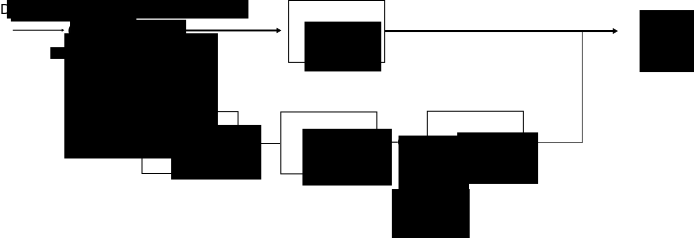
\includegraphics[width=0.5\textwidth]{block_2.eps}
\end{figure}


Our closed-loop is represented as: 

$$ HDD(s) = \frac{G_2(s)}{1 + G_1(s)H(s)F(s)G_2(s)} $$ 

Again, using the specifications for part 2 we get:

\begin{table}[H]
\begin{center}
  \begin{tabular}{ | l | l | l | p{5cm} |}
  \hline
  \textbf{$K_a$} & \textbf{$HDD(s)$}  \\ \hline
  50 & $\frac{0.00255s^2 + 0.05s}{0.0026s^4 + 0.101s^3 + 1.125s^2 + 2.5s}$\\ \hline 
  400 & $\frac{0.00255s^2 + 0.05s}{0.0026s^4 + 0.101s^3 + 2s^2 + 20s}$\\ \hline 
 \end{tabular}
\end{center}
\caption{Closed-Loop System: Unit Step Disturbance}
\end{table}

Using Octave, we observed the response to the unit step reference input. The
Octave code and plots are shown below. 

\matlab{fig4.m}

\begin{figure}[H]
  \caption{Step response for the closed loop system: $K_a = 50$}
  \centering
  \includegraphics[width=0.5\textwidth]{fig4.eps}
\end{figure}

\matlab{fig5.m}

\begin{figure}[H]
  \caption{Step response for the closed loop system: $K_a = 400$}
  \centering
  \includegraphics[width=0.5\textwidth]{fig5.eps}
\end{figure}

\subsubsection*{Task 3C: Satisfying the Performance Specifications}

For this sub-task, a value for $K_a$ was needed to meet performance 
specifications of the system. The specifications are shown in the table below.

\begin{table}[H]
\begin{center}
  \begin{tabular}{ | l | l | l | p{5cm} |}
  \hline
  \textbf{Performance Measure} & \textbf{Specification}\\ \hline 
  Percent overshoot & Less than $5\%$ \\ \hline 
  Settling time ($2\%$ deviation) & Less than 250 ms \\ \hline 
  Maximum Value of response to a unit step disturbance & Less than 
  $5\cdot10^{-3}$ \\ \hline 
 \end{tabular}
\end{center}
\caption{Transient Response Performance Specifications}
\end{table}

After observing the response of the system for varying values of $K_a$ we
concluded that it was not possible to meet all aspects of the specifications
from the proportional compensator. 

The shortest settling time we could get was approximately 0.37 seconds, for
$K_a = 1450$. We noticed a parabolic relationship between $K_a$ and the
settling time. Values smaller, and larger than $K_a = 1450$ gave longer
settling times. Settling time seemed to be the smallest at approximately
$K_a = 1450$.

\matlab{fig6.m}

\begin{figure}[H]
  \caption{Shortest Settling Time Achievable From Compensator: 
  $K_a \approx 1450$, Settling Time $\approx 370$ ms}
  \centering
  \includegraphics[width=0.5\textwidth]{fig6.eps}
\end{figure}

To meet the appropriate overshoot, we set $K_a$ to 200, which
indeed did place the system within the correct specification margins for
overshoot, but placed it outside the bound of the maximum value of the response
 to a unit step disturbance. Increasing $K_a$ higher brought the system
closer to meeting the specification for the maximum bound, but further away from
meeting the overshoot specification. $K_a = 220$ for example, gave a maximum
value just under the required $5\times 10^{-3}$.

The following graphs show how changing $K_a$ from 200 to 220 pushes
the response of the unit step disturbance over the boundary of its
accepted maximum response.

\begin{figure}\centering
  \begin{minipage}{0.5\linewidth}
    \matlab{fig7.m}%
  \end{minipage}%
  \begin{minipage}{0.5\linewidth}
    \matlab{fig8.m}
  \end{minipage}%
\end{figure}

\begin{figure}[H]\centering
  \caption{Unit step disturbance for different $K_a$}
  \begin{minipage}{9cm}
    \includegraphics[width=1.0\textwidth]{fig7.eps}
  \end{minipage}%
  \begin{minipage}{9cm}
    \includegraphics[width=1.0\textwidth]{fig8.eps}
  \end{minipage}
\end{figure}

The root locus Matlab code and plot are shown below:
\matlab{fig13.m}
\begin{figure}[H]
  \caption{Root Locus Plot for HDD(s): We see that for any value of $K$ 
  (highlighted line) we cannot meet all of the requirements}
  \centering
  \includegraphics[width=0.5\textwidth]{fig13.eps}
\end{figure}

In conclusion, this task required building a complete mathematical model for
the HDD Read Head system, and then using this model to meet required
specifications. This task also showed, however, that adding a compensator will
not necessarily change the system to meet all specifications. In part C of
this task, we saw that when adding a compensator we were able to meet certain
specification requirements, but never all of them. This task made an important
observation in showing not all compensators are the same, as tasks later on
will show.

\subsection*{Task 4: Positional and Velocity Sensor}

In this task an alternative output sensor was considered, that measures the
position as well as the velocity of the head reader. Its represented by $H(s)
= 1 + K_1s$. This task, like Task 3C, relied in our understanding from class of
manipulating transfer functions with compensators. However unlike Task 3C, we
now have control over both poles and zeroes. Our system transfer function is
now the same as in task 3A, but with a different value for $H(s)$:

$$HDD(s) = \frac{F(s)G_1(s)G_2(s)}{1 + F(s)G_1(s)G_2(s)H(s)}$$

The system now has two different K values that can be changed in order to meet
the specifications from Table 4. After trying different K values we found that
$K_a = 370$ and $K_1 = 0.04$ enabled the system to satisfy all requirements.
A value of $K_1 = 0.04$ gave our system a zero at $-25$. Below, the graphical
analysis of the system (with sensor) is shown, as well as specific values.

%TODO Maybe put these side by side like task 3C?

\matlab{fig14.m}

\begin{figure}[H]
  \caption{System's unit Step response with Positional Velocity Sensor, with response
  time and percent overshoot within specification} 
  \centering
  \includegraphics[width=0.5\textwidth]{fig14.eps}
\end{figure}

\matlab{fig15.m}

\begin{figure}[H]
  \caption{System's unit Step disturbance with Positional Velocity Sensor, with
  maximum value of response within specification}
  \centering
  \includegraphics[width=0.5\textwidth]{fig15.eps}
\end{figure}


From the above graphs, the system shows the following values in its response:

\begin{table}[H]
\begin{center}
  \begin{tabular}{ | l | l | l | p{5cm} |}
  \hline
  \textbf{Performance Measure} & \textbf{Specification}\\ \hline
  Percent overshoot & 0.134\% \\ \hline
  Settling time ($2\%$ deviation) & 243ms \\ \hline
  Maximum Value of response to a unit step disturbance & $3\cdot10^{-3}$\\ \hline 
 \end{tabular}
\end{center}
\caption{Response Performance from Positional Velocity Sensor $H(s) = 1 +
0.004 s$}
\end{table}

All above values were within the specifications of the system, and all were
achieved with the same K values, unlike the system in Task 3.

In conclusion, it was also found that for this system, having a zero less than
-20 enabled the creation of a system that was able to meet the specifications.
This was because a zero at that particular location caused the poles of the
system to break out towards the left, and into the desired region (as set by
the specifications).

This task showed how having control of both zeros and poles of the system gave
the engineer of the system (us) more control. Without the ability to add a
zero to the system and changing its position, the system would not have been
able to meet the specifications, as was the case in Task 3C.

\subsection*{Task 5: The PID Compensator}

In this task we used the PID Compensator architecture, as discussed in class,
to manipulate the plant such that the system can meet the desired specifications.
The particular specification of this task also reverted the sensor back
to $H(s) = 1$, while the controller now assumes a transfer function of the form

$$ F(s) = K_1 + \frac{K_2}{s}  + K_3s $$

\noindent
where $K_2 = 0$ because the plant (arm) inherently has an integrating
term. $G_1(s)$ and $G_2(s)$ remained the same. The project description 
furthermore states that $\frac{K_1}{K_3} = 1$. As in the previous Tasks, our 
system transfer function is still of the form:

$$HDD(s) = \frac{F(s)G_1(s)G_2(s)}{1 + F(s)G_1(s)G_2(s)H(s)}$$

Using the PID Compensator the system was not able to achieve a settling time
of less than 250 ms, as described in the spec. However, other design
specifications were able to be met. 

When carrying out Matlab/Octave calculations, we were not able to always
measure exact settling time, but in all of the graphs, it is pictorially clear
that for any value of $K$ that the settling time was greater than 1 second, thus
not within the 250 ms requirement. From varying $K$, it was noticed that $K$
needed to be less than 210, for the disturbance response to be below the maximum
disturbance. 

\matlab{fig16.m}

\begin{figure}[H]
  \caption{Step Disturbance showing the highest value of $K$ such that the
  system stays within the Maximum Disturbance value}
  \centering
  \includegraphics[width=0.5\textwidth]{fig16.eps}
\end{figure}

The maximum $K$ value which we could reach in order to be below
the maximum overshoot was 643. The overshoot keeps increasing for any larger
value of $K$. 

\matlab{fig17.m}

\begin{figure}[H]
  \caption{Step response showing the highest value of $K$ such that the
  system stays within the Maximum Percent Overshoot. Note the extremely long
  settling time}
  \centering
  \includegraphics[width=0.5\textwidth]{fig17.eps}
\end{figure}

Unfortunately both aforementioned values of $K$ were too low to
meet the settling time requirement, and although raising $K$ would have given
a lower settling time the overshoot increases dramatically, as shown below: 

\matlab{fig18.m}

\begin{figure}[H]
  \caption{Dramatic improvement in the step response for higher values of $K$:
  $K = 6000$}
  \centering
  \includegraphics[width=0.5\textwidth]{fig18.eps}
\end{figure}

In Conclusion, this PID Compensator unfortunately did not meet all requirements
either. Although it met more requirements than the Proportional Compensator in
Task 3, it did not perform as well as the Positional and Velocity Sensor in
Task 4. For varying values of $K$, we could only meet 2 out of the 3 requirements.
For $K < 210$, both the Percent Overshoot and Maximum Disturbance values were
met, but not Settling Time. For much larger values of $K$ (6000 for example,
as shown above), Settling Time was met, but not Maximum Disturbance. This 
Compensator can still be used however, depending on which Performance 
Specification can be relaxed. If a value of $K$ was needed to be chosen for 
this System exactly, we would recommend sacrificing Overshoot rather than
Disturbance, so as to create a more predictable output.

\subsection*{Task 6: Refined Arm Model and Frequency Response Characterization}

The HDD architecture has been revised again, so that now the flexure spring
is no longer assumed to be rigid. This task attempts to design a sensor for the
HDD using this new model, using our knowledge of settling time and overshoot
as learned in class, and understanding of gain and phase margins.

\subsubsection*{Task 6A: Determining the Unit Step Response}

The spring load system is now added to the block diagram as shown below:

\begin{figure}[H]
  \centering
  \caption{Refined System Model}
  \includegraphics[width=0.5\textwidth]{block_3.eps}
\end{figure}

This is the transfer function for the (isolated) spring load system:

$$G_3 = \frac{1}{1 + \frac{2\zeta s}{\omega_n} + \frac{s^2}{\omega_n^2}}
      = \frac{1}{2.814\times 10^{-9} ~ s^2 + 3.183\times 10^{-5} ~ s + 1}$$

\noindent
where given values for $\zeta$ and $\omega_n$ have been filled in.
The step response of this system is observed using the following code:

\matlab{fig9.m}

\begin{figure}[H]
  \caption{Step response of spring load system}
  \centering
  \includegraphics[width=0.5\textwidth]{fig9.eps}
\end{figure}

\subsubsection*{Task 6B: Examining the Magnitude}

The closed loop system transfer function for the entire system changes
to the following form:

$$HDD(s) = \frac{F(s)G_1(s)G_2(s)G_3(s)}{1 + F(s)G_1(s)G_2(s)G_3(s)H(s)}$$

\noindent
where $H(s) = 1$.  The parameter $K_1 = K_3$ is to be varied from 100
to 1000, while the Bode plot of the closed loop system is observed
below.

\matlab{fig10.m}

\begin{figure}[H]\centering
  \caption{bode plots for varying $K_1 = K_3$}
  \begin{minipage}{9cm}
    \includegraphics[width=1.0\textwidth]{fig10.eps}
  \end{minipage}%
  \begin{minipage}{9cm}
    \includegraphics[width=1.0\textwidth]{fig11.eps}
  \end{minipage}\\
  \begin{minipage}{9cm}
    \includegraphics[width=1.0\textwidth]{fig12.eps}
  \end{minipage}%
  \begin{minipage}{9cm}
    \includegraphics[width=1.0\textwidth]{fig12b.eps}
  \end{minipage}
\end{figure}

A resonant peak appears for values of $K_1 = K_3$ as low as about 500.
As $K_1$ ($K_3$) is increased, the magnitude of the peak increases
and moves towards the right.

\subsubsection*{Task 6C: Finding a range for $K$}

For values of $K_1$ ($K_3$) below 371, the system functions correctly,
but does not meet the transient specifications.  It does not
overshoot, but it also does not have a sufficiently short 2\% settling
time.  For $K_1 = K_3 = 371$, the 2\% settling time is about 940 ms
(larger than the required 250 ms).

%TODO add graphs

However, by breaking the $K_1 = K_3$ constraint, setting $K_1 = 371$
and $K_3 = 853$, the response is closer to meeting the specifications.

\begin{table}[H]
\begin{center}
  \begin{tabular}{ | c | c | c | c |}
  \hline
  $K_1$ & $K_3$ & \% overshoot & settling time (ms) \\ \hline
  371   &   853 &           12 &                250 \\ \hline
  371   &   631 &            5 &                650 \\ \hline
 \end{tabular}
\end{center}
\caption{sets of parameters that satisfy at least one condition}
\end{table}

\begin{figure}\centering
  \begin{minipage}{0.5\linewidth}
    \matlab{fig19a.m}%
  \end{minipage}%
  \begin{minipage}{0.5\linewidth}
    \matlab{fig19b.m}
  \end{minipage}%
\end{figure}

\begin{figure}[H]\centering
  \caption{closed loop step responses, making different sacrifices}
  \begin{minipage}{9cm}
    \includegraphics[width=1.0\textwidth]{fig19a.eps}
  \end{minipage}%
  \begin{minipage}{9cm}
    \includegraphics[width=1.0\textwidth]{fig19b.eps}
  \end{minipage}
\end{figure}


\subsubsection*{Task 6D: Gain and Phase Margins}

\section*{Conclusion}

In conclusion, this project designed and observed several different controllers
for the Hard Disk Drive system. Not all controllers met the necessary
specifications, and some performed better on certain specifications than others.

In the end, the controllers that performed best were the Positional and Velocity
Sensor (Task 4), and the PID Compensator (Task 5). However, only 2 of the 3
specifications were able to be met for the PID Compensator, and therefore the
recommendation is to use the Positional and Velocity Sensor.

The block diagram for the Positional and Velocity Sensor is shown again, below:

\begin{figure}[H]
  \centering
  \caption{Block Diagram of HDD system}
  \includegraphics[width=0.5\textwidth]{block_1.eps}
\end{figure}

\begin{table}[H]
  \begin{center}
    \begin{tabular}{ | l | l | l | p{5cm} |}
    \hline
    \textbf{Block} & \textbf{Mathematical Model} \\ \hline
    Controller & $F(s) = K_a$ \\ \hline 
    Motor Coil& $G_1 = \frac{K_m}{Ls + R}$ \\ \hline
    Arm Load & $G_2 =  \frac{1}{s(Js + b)}$ \\ \hline
    Sensor & $H(s) = 1 + K_1s$ \\ \hline
   \end{tabular}
 \end{center}
 \caption{Block Architecture Description}
\end{table}

\begin{table}[H]
  \begin{center}
    \begin{tabular}{ | l | l | l | p{5cm} |}
    \hline
    \textbf{$K$} & \textbf{Value} \\ \hline
    $K_a$ & $370$ \\ \hline
    $K_1$ & $0.04$ \\ \hline
   \end{tabular}
 \end{center}
 \caption{Values of $K$ for the Architecture}
\end{table}

The closed loop transfer function of the entire system, as mentioned in Task 4,
came out to be:

$$HDD(s) = \frac{F(s)G_1(s)G_2(s)}{1 + F(s)G_1(s)G_2(s)H(s)}$$

It was shown in Task 4 that all requirements were met. The table showing the
performance results is shown below for convenience:

\begin{table}[H]
\begin{center}
  \begin{tabular}{ | l | l | l | p{5cm} |}
  \hline
  \textbf{Performance Measure} & \textbf{Specification}\\ \hline 
  Percent overshoot & Less than $5\%$ \\ \hline 
  Settling time ($2\%$ deviation) & Less than 250 ms \\ \hline 
  Maximum Value of response to a unit step disturbance & Less than 
  $5\cdot10^{-3}$ \\ \hline 
 \end{tabular}
\end{center}
\caption{Transient Response Performance Specifications}
\end{table}

Note that for this particular $K_1$, $K_a = 370$ was the minimum value of $K$
such that the settling time would be under 250 ms. For higher values of $K$ the
settling time goes down, without affecting any of the other parameters, although
the Gain Margin does get lower for very large values of $K_a$. We can see the
Gain and Phase Margins below:


\matlab{fig20.m}

\begin{figure}[H]
  \caption{Phase and Gain Margins for the system}
  \centering
  \includegraphics[width=0.5\textwidth]{fig20.eps}
\end{figure}

In the end, the Positional and Velocity Sensor enabled us the system to stay
within the specified requirements. The Gain Margin was also acceptable. The Phase
Margin was high at $180 \degree$, and its frequency was not able to be calculated
by Matlab/Octave. The $K_a$ chosen for this design was rather conservative at
$K_a = 370$, future designs following this model could raise $K_a$ to 1000 to
achieve a settling time of 165 ms, although lowering the Gain Margin. If in the
future, there is more constraint on the Gain Margin, a range for $K_a$ could be
narrowed down even further. However the current values for the Positional and
Velocity Sensor meet all specifications, and is the sensor this project
recommends be used in the hard disk drive.

\end{document}
